\chapter{Background Research}\glsresetall
\label{cha:Research}
As a part of the implementation of a viable grasping point of objects in an environmental setting a research of state of the solutions of both object tracking and detection is necessary as well as researching full existing solutions.

\section{Object Detection and Tracking}
In order to get some understanding of the state of the art technologies used the research in split into multiple sections for different areas in the process of teaching a robot to pick groceries from a shelf.

\subsection{Object Detection}
The aim of generic object detection is to locate and classify an object in an image, sometimes including a bounding box on objects with a confidence of existence in the image. In general there are two approaches to object detection namely region proposal, which follows the traditional object detection pipeline and then classifying the each proposal into different object categories. The other approach is the regression or classification based approach by adopting a unified framework to achieve final results \citep{zhao}.
\cite{zhao} presents several solutions of both approaches and have also made a small roadmap of different popular solutions up until 2017. This is shown in \autoref{fig:deep_roadmap}.


\begin{figure}[H]
  \centering
  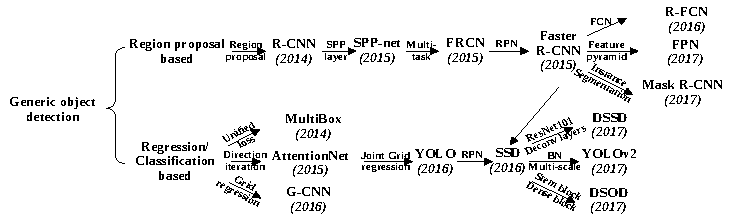
\includegraphics[widht=\textwidth]{deep_roadmap.pdf}
  \caption{Small roadmap of different popular solutions up until 2017 \citep{zhao}}
  \label{fig:deep_roadmap}
\end{figure}

I'm confused by this..
